\chapter{UML Examples}
\section{Ein einfaches Zeichnungsprogramm}
Es soll ein Programm zur interaktiven Erstellung 
von einfachen Zeichnungen entwickelt werden.
Das Programm soll nach dem Aufstarten 
ein leeres Fenster anzeigen, in welchem der Benutzer
durch Verschieben des Mauszeigers
bei gedr\"uckter Maustaste Linienz\"uge erzeugen kann, die 
in bestimmter Strichdicke und Farbe unmittelbar der Bewegung des 
Mauszeigers folgend angezeigt werden.
\newslide
\subsection{Bestimmung der Klassen}
Aus der Problembeschreibung können die folgenden Substantive
und damit potentiellen Klassen gefunden werden. Aus Konsistenzgründen
verwenden wir englische Begriffe:\\
\begin{tabular}{llcll}
          & englisch & Verwendung & Qt-Basisklasse & Swing\\
\hline
 Programm & Application & \OK & QApplication  & JApplet\\
 Erstellung & Creation &    &  &\\
 Zeichnung & Drawing, Document &  \OK &  & \\
 Aufstarten & Start-up & &  &\\
 Fenster & Window, View & \OK &  QFrame & JPanel\\
 Zeichenfläche & DrawingArea & \OK & & \\
 Verschieben & Move &   & &\\
 Mauszeiger & Mouse pointer & & &\\
 Maustaste & Mouse button & & &\\
 Benutzer & User &         & & \\
 Linienzug & Line stroke & \OK & &\\
 Bewegung & Move & & & \\
\end{tabular}
\subsection{Klassendiagramm}\ \\
%
\ifslides
\begin{center}
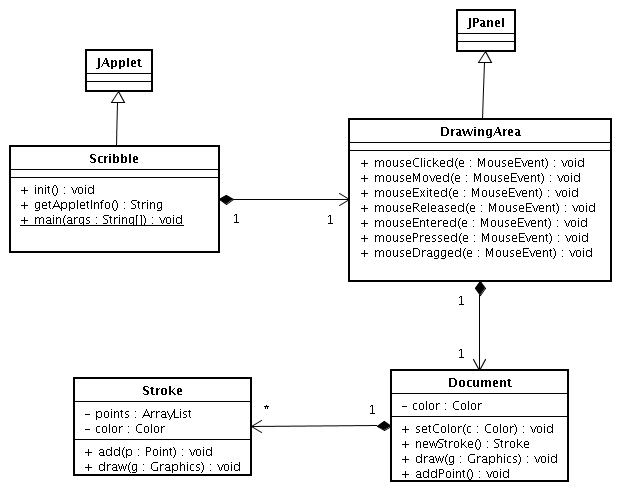
\includegraphics[width=0.65\linewidth]{examples/Scribble/doc/scribble-classdiagram}
\end{center}
\else
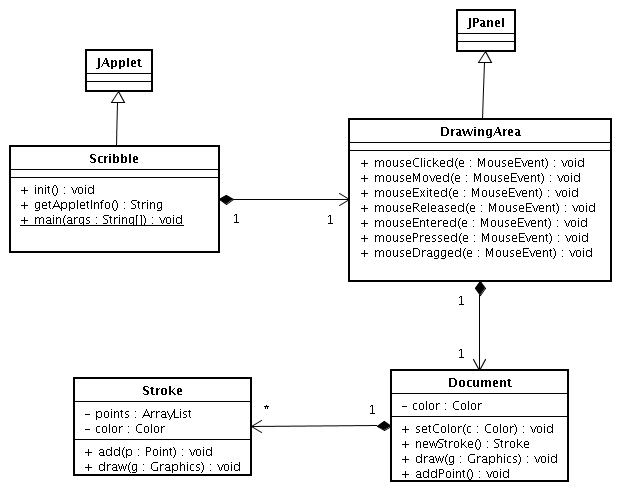
\includegraphics[width=0.9\linewidth]{examples/Scribble/doc/scribble-classdiagram}
\fi
\subsection{Sequenzdiagramm} Zeichnen einer Linie\\[2ex]
%
\ifslides
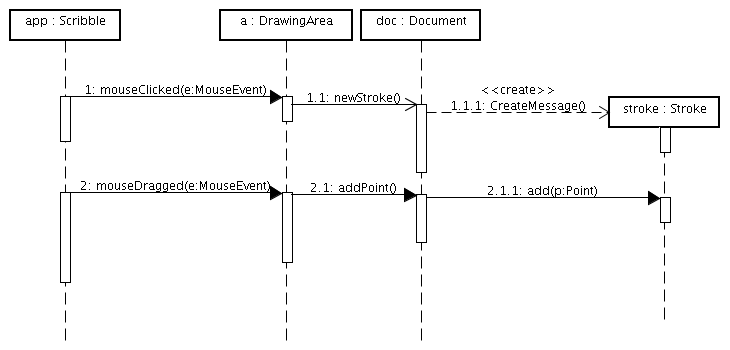
\includegraphics[width=0.9\linewidth]{examples/Scribble/doc/scribble-seq}
\else
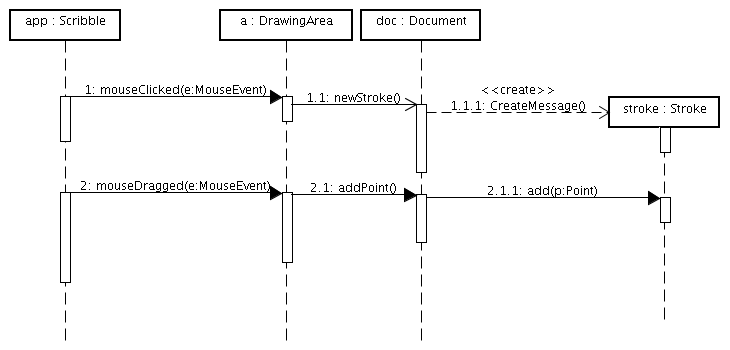
\includegraphics[width=\linewidth]{examples/Scribble/doc/scribble-seq}\\[2ex]
\newpage
\subsection{Zustandsdiagramm} \ \\[2ex]
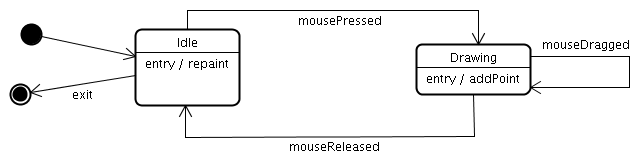
\includegraphics[width=0.9\linewidth]{examples/Scribble/doc/scribble-statechart}
%
\subsection{Das Hauptprogramm}
%Typisch für Window-basierte Programme werden im
Im Hauptprogramm  wird die Applikation und das Zeichnungsfenster
instantiiert und miteinander verknüpft. Anschliessend erfolgt
die Anzeige des Fensters und das Programm springt in die
 Ereignisbehandlungsschleife. Hier handelt
es sich um die Ereignisse: mousePressed, mouseDragged, mouseReleased und
paintComponent,
bei deren Auftreten die entsprechenden Methoden des DrawingArea-Objekts
aufgerufen werden.
\fi
\newslide
\begin{lstlisting}[language=java]
public class Scribble {
  /**
  * Create the GUI and show it.  For thread safety, this method
  * should be invoked from the event-dispatching thread.
  */
  private static void createAndShowGUI() {
    JFrame.setDefaultLookAndFeelDecorated(true);
    JFrame frame = new JFrame("Scribble");
    frame.setDefaultCloseOperation(JFrame.EXIT_ON_CLOSE);
    
    Scribble scribble = new Scribble();
    DrawingArea drawingArea = new DrawingArea();
    frame.getContentPane().add( drawingArea );
    
    frame.pack();
    frame.setVisible(true);
  }
  
  public static void main(String[] args) {
    javax.swing.SwingUtilities.invokeLater(new Runnable() {
      public void run() { createAndShowGUI(); }
    });
  }
}
\end{lstlisting}
\newpage
\begin{lstlisting}[language=java]
public class DrawingArea extends JPanel
   implements MouseInputListener {
        
     private Document document;

     public DrawingArea() {
       document=new Document();
       addMouseListener(this);
       addMouseMotionListener(this);
     }

     protected void paintComponent(Graphics g) {
       document.draw(g);
     }

     //Methods required by the MouseInputListener interface.
     public void mouseClicked(MouseEvent e) { }
     public void mouseMoved(MouseEvent e) { }
     public void mouseExited(MouseEvent e) { }
     public void mouseReleased(MouseEvent e) { }
     public void mouseEntered(MouseEvent e) { }
     
     public void mousePressed(MouseEvent e) { 
       document.newStroke();
       document.addPoint( new Point(e.getX(),e.getY()) );
     }
     
     public void mouseDragged(MouseEvent e) {
       document.addPoint( new Point( e.getX(), e.getY() ) );
       repaint();
     }
   }
\end{lstlisting}
\newpage
\begin{lstlisting}[language=java]
public class Document {
    ArrayList<Stroke> strokes=null;
    Stroke stroke;
    Color  color;

    Document(){
        strokes = new ArrayList<Stroke>();
        color = Color.blue;
    }

    public void setColor( Color c ){
        color = c;
    }

    public Stroke newStroke(){
        stroke = new Stroke(color);
        strokes.add( stroke );
        return stroke;
    }

    public void addPoint( Point p ){
      stroke.add(p);
    }

    public void draw( Graphics g ){
        Iterator<Stroke> i = strokes.iterator();
        while( i.hasNext() ){
            Stroke s=i.next( );
            s.draw(g);
        }
    }
}
\end{lstlisting}
\newpage 
\begin{lstlisting}[language=java]
public class Stroke {
    ArrayList<Point> points;
    Color  color;

    public Stroke(Color c){
        points = new ArrayList<Point>();
        color = c;
    }

    /** adds a point to the stroke
     * @param p point to be added
     */
    public void add( Point p ){
        points.add( p );
    }
    /** draws the stroke
     * @param g graphics object
     */
    public void draw( Graphics g ){
        if( points.size()<1 )
            return;

        g.setColor( color );
        Iterator<Point> i=points.iterator();
        Graphics2D g2d = (Graphics2D)g;

        Point p1 = i.next();
        while( i.hasNext() ){
            Point p2 = i.next();
            g2d.drawLine( p1.x, p1.y, p2.x, p2.y );
            p1 = p2;
        }
    }
}
\end{lstlisting}
%
\newpage
\section{Die Türme von Hanoi}
Einer Legende gemäss mussten indische Mönche 64 mit abnehmendem Durchmesser
über\-einan\-der ge\-sta\-pel\-te Scheiben von einem heiligen
Ort zu einem andern bringen. Da die Scheiben sehr zerbrechlich waren, durfte nur eine
aufs Mal getragen werden. Und zudem durfte nie eine kleinere Scheibe unter einer
grösseren zu liegen kommen. Ein dritter Ort war als Zwischenlager der Scheiben zugelassen.

Die Legende erzählt weiter, dass der Tempel längst in Staub zerfallen sein und die Erde
aufgehört haben wird zu existieren, bevor die Mönche ihren Auftrag erfüllt hätten.

Entwickeln Sie ein Programm, mit dem sich diese Behauptung überprüfen lässt. 
Der Anwender soll mit dem Mauszeiger die beiden Türme, zwischen welchen anschliessend 
jeweils eine Scheibe verschoben wird auswählen können. 
Ausserdem soll es möglich sein, die Anzahl der Scheiben vorgeben zu können.

Existiert ein Algorithmus, der diese Aufgabe mit der geringst 
möglichen Anzahl Verschiebungen löst?
\subsection{Beschreibung der Anwendungsfälle}
Wir können für das beschriebene Problem die folgenden Anwendungsfälle finden:
\begin{enumerate}
\item Das Programm aufstarten. Es wird ein Fenster angezeigt, welches drei
     gleich\-mässig nebeneinander angeordnete Türme enthält. Die voreingestellte Anzahl 
     Scheiben liegen mit abnehmender Breite übereinandergestapelt auf dem
     ersten Turm, der sich in der linken Bildhälfte befindet.
\item Die Scheiben des ersten Turmes auf den mittleren verschieben:
  \begin{enumerate}
   \item  Den Mauszeiger zum Turm bewegen, dessen oberste Scheibe verschoben werden
        soll.
   \item  Den linken Mausknopf drücken. Die oberste Scheibe dieses Turms
               wird nun selektiert.
   \item Den Mauszeiger zum Turm verschieben, wo die Scheibe abgelegt werden soll.
   \item Die linke Maustaste drücken. Die selektierte Scheibe wird nun auf
      die oberste Position dieses zweiten Turms verschoben, sofern darunter
      nicht bereits eine Scheibe mit kleinerem Durchmesser liegt.
   \item Die Schritte (a) bis (d) werden solange wiederholt, bis
       alle Scheiben des Ursprungsturmes in derselben Reihenfolge 
       am Zielort aufgestapelt sind.
  \end{enumerate}
\item Die Ausgangssituation wiederherstellen.
\item Den implementierten Algorithmus ausführen lassen.
\item Das Programm beenden.
\end{enumerate}
\newpage
\subsection{Anwendungsfall-Diagramm}
\begin{center}
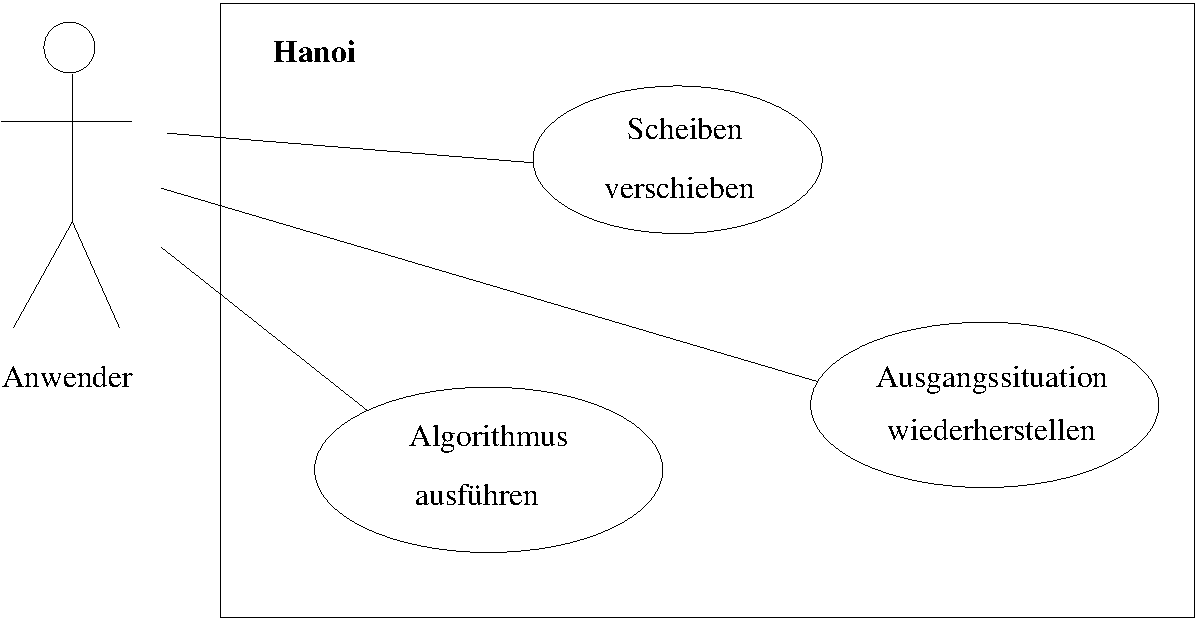
\includegraphics[width=\linewidth]{examples/xfig/hanoi-usecase}
\end{center}
\ifslides
\newpage
\fi
\subsection{Entwurf der grafischen Oberfläche}\ \\[2ex]
\ifslides
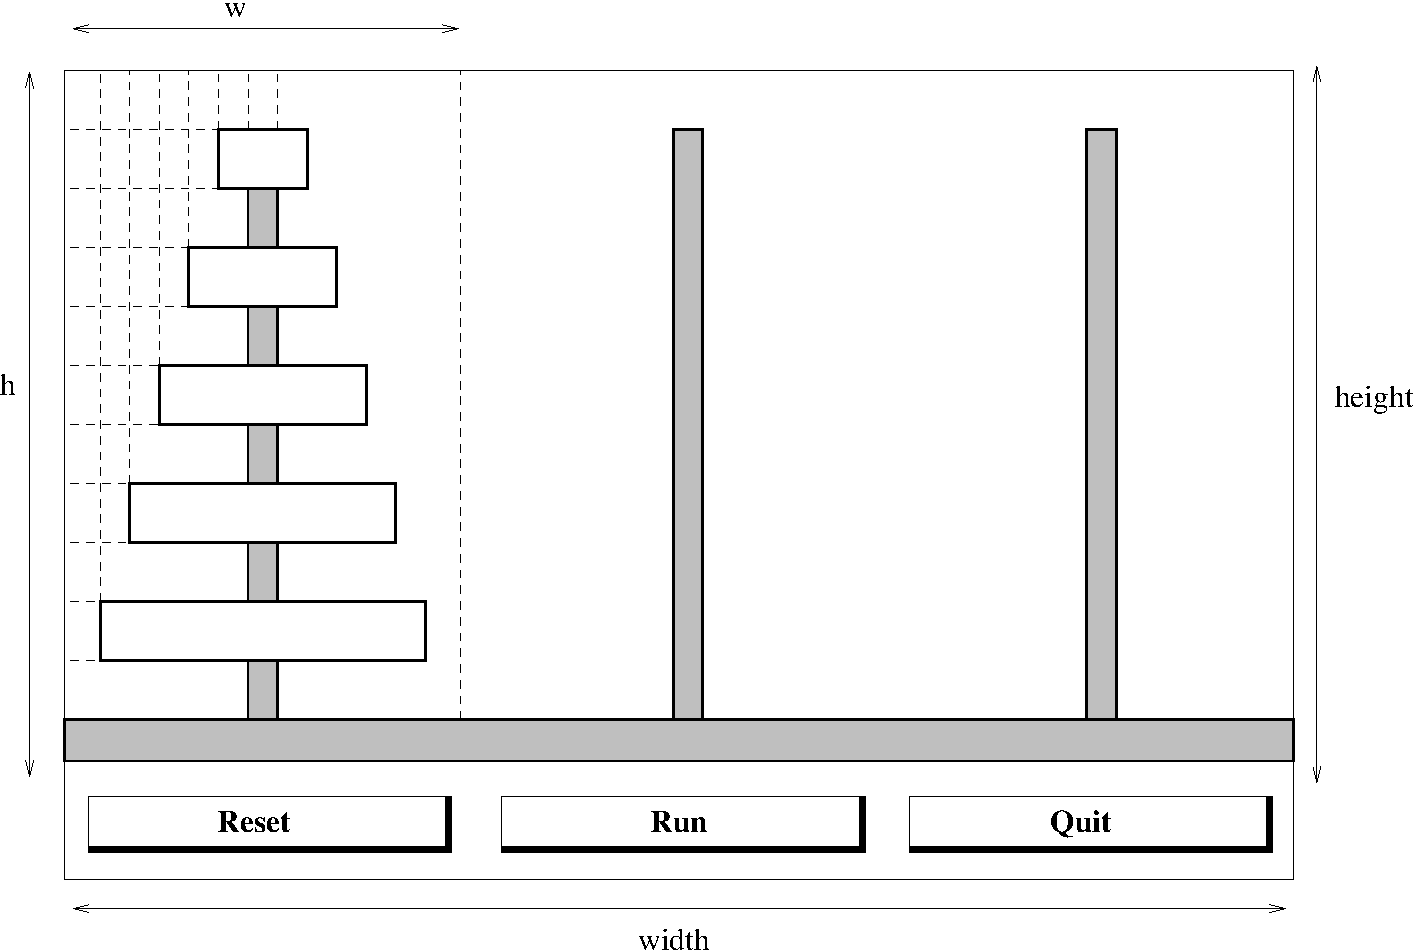
\includegraphics[width=0.8\linewidth]{examples/xfig/gui-hanoi}\\
\else
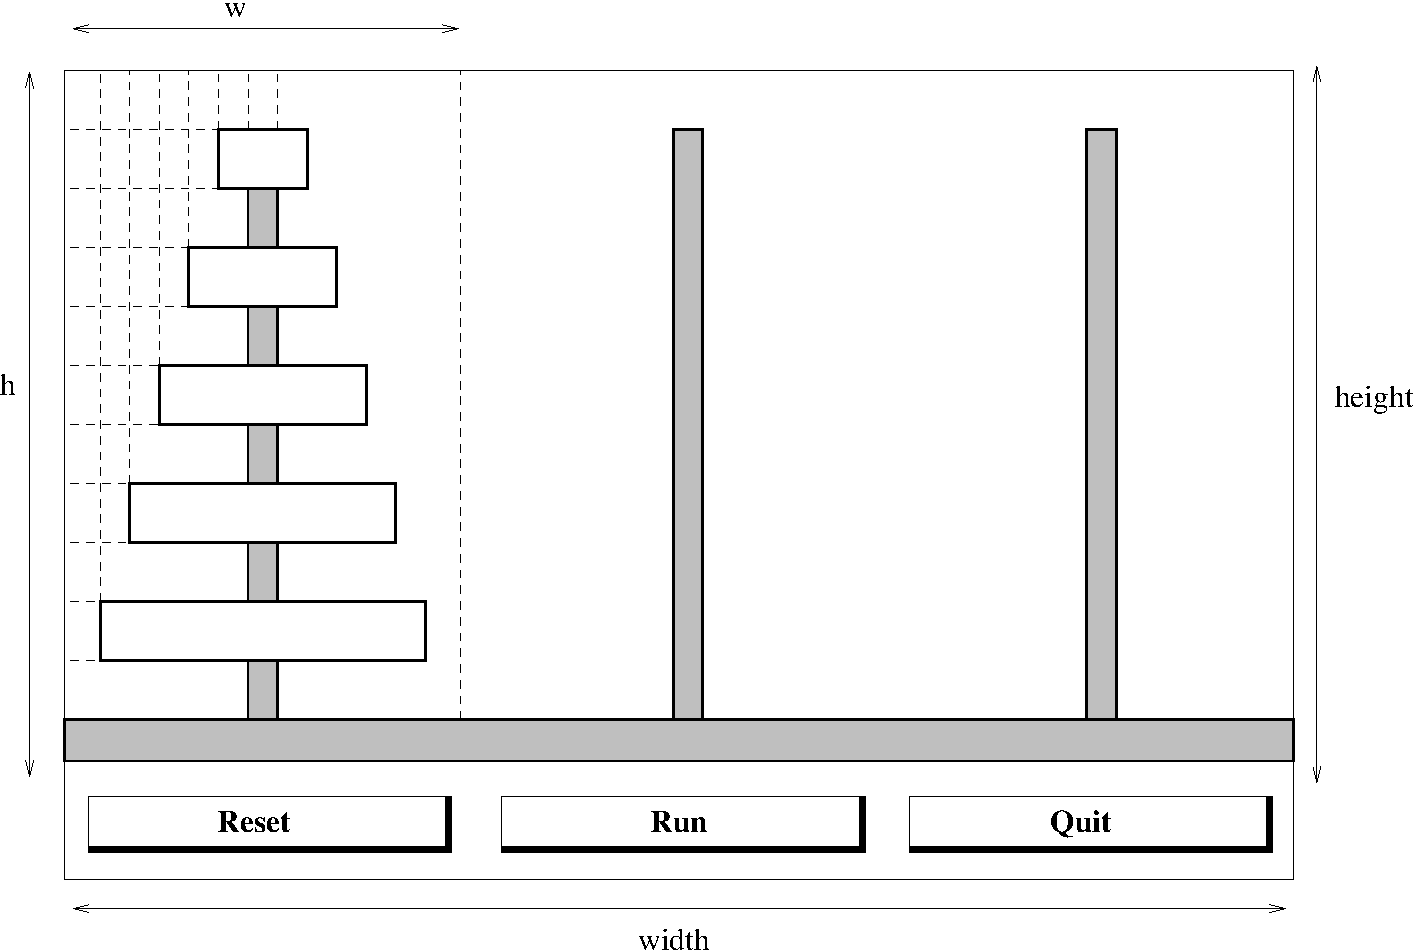
\includegraphics[width=\linewidth]{examples/xfig/gui-hanoi}
\fi
Alle zur Bedienung erforderlichen Elemente sollen, wie in obiger Abbildung
dargestellt, in einem einzigen Fenster enthalten sein. 
Dieses Fenster besteht aus einem Zeichnungsfeld,
in welchem die Türme und Scheiben dargestellt sind mit darunter 
angeordnetem Aktionsfeld, welches die Schaltflächen
\begin{description}
\item[Reset:] zur Wiederherstellung der Ausgangssituation, 
\item[Run:] zur Ausführung des Algorithmus' und 
\item[Quit:] zum Verlassen des Programms
\end{description} enthält. 

Die Elemente sollen
unabhängig von der jeweiligen Grösse, die der Anwender jederzeit mit dem Mauszeiger
verändern kann, stets die zur Verfügung stehende Fensterfläche
ausfüllen. Aus der Abbildung
können folgende Darstellungsregeln festgehalten werden:
\begin{enumerate}
\item Jedes Zeichnungselement Turm, Scheibe und Bodenplatte wird durch ein mit einer
  bestimmten Farbe gefülltes Rechteck dargestellt.
\item Jede Scheibe ist eine Zeichnungseinheit hoch und $2\cdot i + 1$ Einheiten breit,
  wobei i die mit 1 beginnende und von oben nach unten inkrementierte Lageposition
  der Scheibe kennzeichnet. 
\item Der Zwischenraum zwischen zwei Scheiben beträgt eine Zeichnungseinheit.
\item Die Bodenplatte ist eine Zeichnungseinheit hoch und genau so breit wie
  die Zeichnungsfläche.
\item Ein Turmstab ist eine Zeichnungseinheit breit und genau so
 hoch wie alle übereinander
  liegenden Scheiben mit ihren Zwischenräumen.
\item Die Turmbreite ist um 2 Einheiten grösser als die Breite der grössten
  Scheibe. 
\item Die Zeichnungsfläche ist in der Höhe eine Einheit grösser als die Summe
  der Turmhöhe und der Dicke der Bodenplatte.
\end{enumerate}
Daraus ergeben sich für die Turmhöhe $h$ und Turmbreite $w$ 
in Abhängigkeit der Anzahl Scheiben $n_{disks}$
die folgenden Beziehungen:
\begin{eqnarray}
 h & = & 2\cdot n_{disks} + 3\\
 w & = & 2\cdot n_{disks} + 3
\end{eqnarray}
Wenn die Fensterabmessungen $width$ x $height$ Pixel betragen, ergibt sich damit für die
Zeichnungseinheiten $t_x$ und $t_y$ in x- und y-Richtung:
\begin{eqnarray}
t_x & = & w/\mbox{width} = \left(2\cdot n_{disks} + 3\right)/\mbox{width}\\
t_y & = & h/\mbox{height} = \left(2\cdot n_{disks} + 3\right)/\mbox{height}
\end{eqnarray}
\ifslides
\newpage
\fi
Die sich an $p$-ter Position auf dem $k$-ten Turm befindende Scheibe $d$ kann
demnach wie folgt gezeichnet werden:
\begin{lstlisting}
int width = 2*d + 1;        // Breite der Scheibe
int posx  = (ndisks+1) * k; // x-Koordinate des Turmes k
int posy  = ( p + 1 );      // y-Koordinate der Position p
g.fillRect( (posx-(width-1)/2)*tx, posy*ty, width*tx, ty );
\end{lstlisting} 
%%%
\newpage
\subsection{Sequenzdiagramm} Verschieben einer Scheibe\\[2ex]
\ifslides
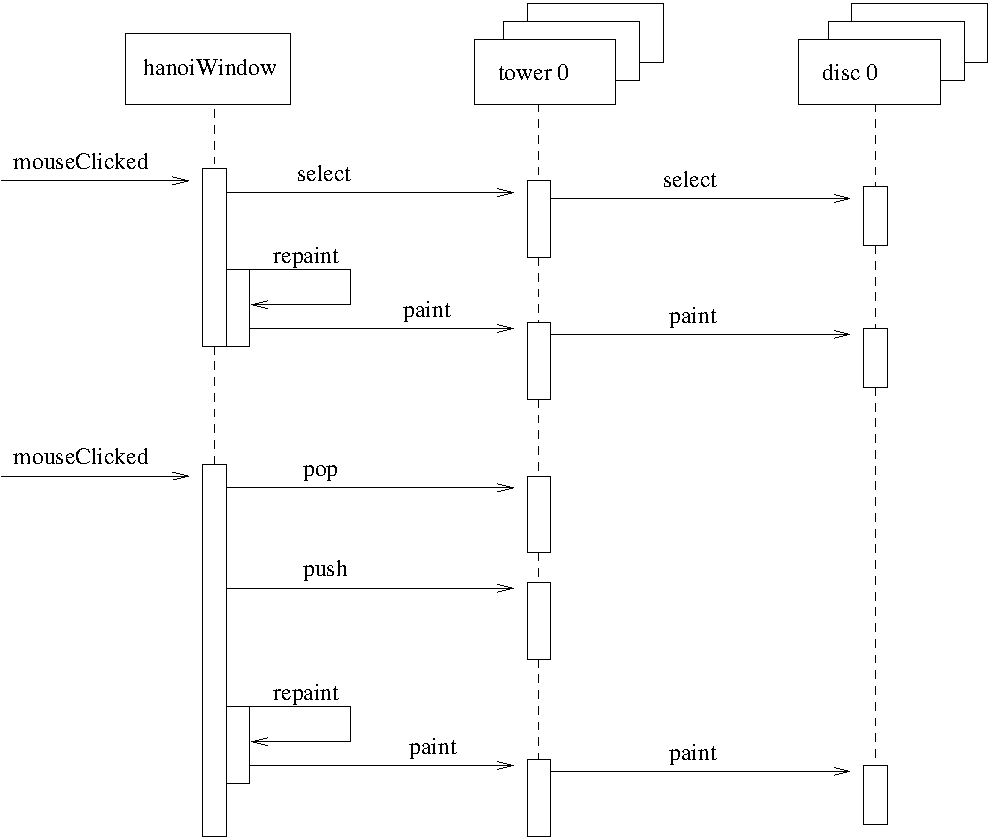
\includegraphics[width=0.6\linewidth]{examples/xfig/hanoi-seqdiag}
\else
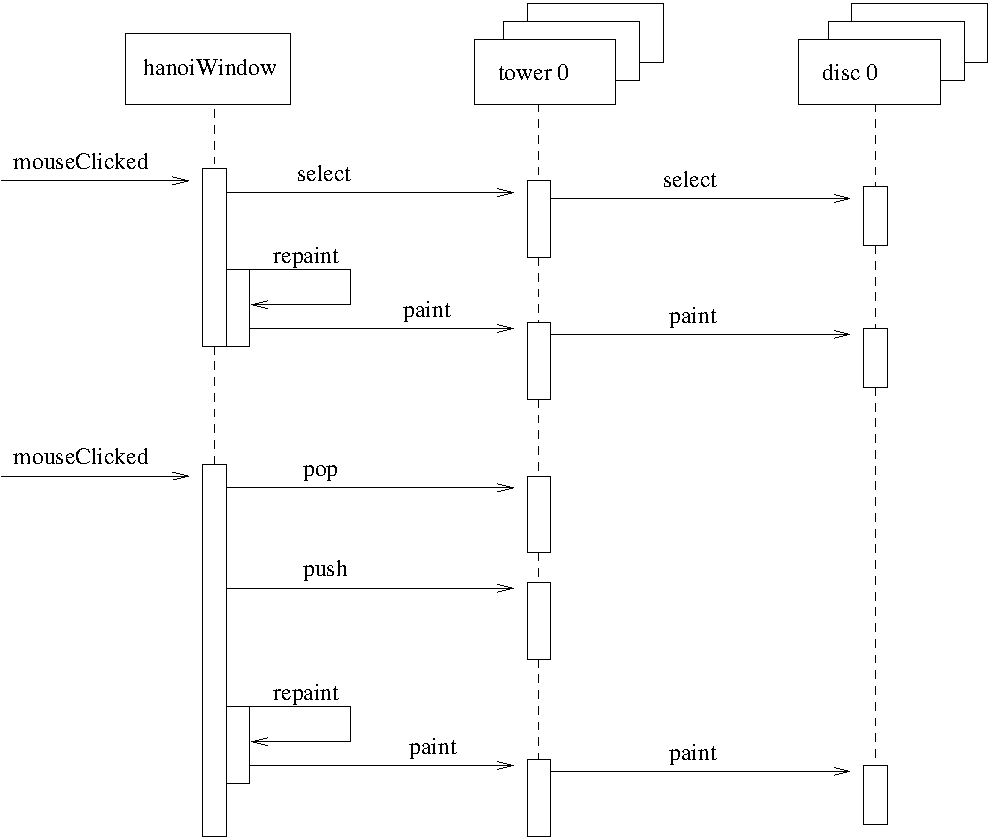
\includegraphics[width=\linewidth]{examples/xfig/hanoi-seqdiag}
\fi
\subsection{Klassendiagramm}\ \\[2ex]
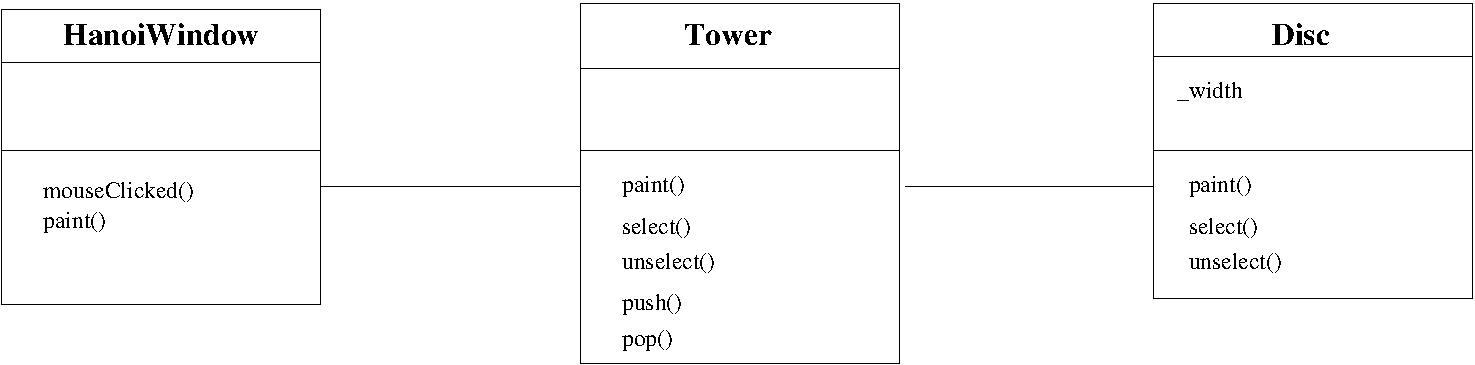
\includegraphics[width=\linewidth]{examples/xfig/hanoi-classdiag}
%
\newpage
\section{Aufgaben}
\begin{enumerate}
%
\item Skizzieren Sie ein Use-Case-Diagramm für
  \begin{enumerate}
  \item ein Fernseher-Fernsteuergerät
  \item eine Dateiverwaltungssoftware
  \item einen Geldautomaten
  \end{enumerate}
\newslide
\item Eine Stoppuhr soll folgende Eigenschaften aufweisen:
\begin{enumerate}
  \item Die Stoppuhr kann ein- und ausgeschaltet werden.
  \item Die Stoppuhr kann gestartet und gestoppt werden. Nach dem
  Stopp wird die abgelaufene Zeit zwischen Start und Stopp angezeigt.
  \item Nach dem Start kann eine Zwischenzeit angezeigt werden.
   Die Uhr läuft im Hintergrund weiter. Nun kann entweder die
   Anzeige von der Zwischenzeit auf die Anzeige 
   der aktuell abgelaufenen Gesamtzeit gewechselt werden
   oder die im Hintergrund laufende Uhr kann angehalten werden,
   ohne dass sich die Anzeige ändert. Im letzten Fall
   wird nach einem weiterem Knopfdruck die vergangene 
  Gesamtzeit angezeigt.
  \item Die zwischen Start und Stopp vergangene Zeit kann
   bei gestoppter Uhr und Anzeige der vergangenen Gesamtzeit
   auf Null zurückgesetzt werden.
 \item Die Uhr besitzt zwei Druckknöpfe, die nicht gleichzeitig
  gedrückt werden können, und eine vierziffrige Anzeige.
% Source: Dr. Hans-Michael Windisch, FH Ingolstadt ?
\end{enumerate}
\newslide
\item Ein Schweizer Hersteller hat ein Telefonsystem im Angebot, bei welchem
  bis zu 6 schnurlose Handgeräte an jeweils einer Feststation betrieben werden
  können. Jedes Handgerät kann bis zu 150 Telefonbucheinträge mit Name und
  Rufnummer 
  speichern. Wenn zwei oder mehr Handgeräte an der Feststation angemeldet sind,
  kann das gesamte Telefonbuch oder einzelne Einträge von einem Handgerät
  auf ein anderes übertragen werden. Man geht dabei wie folgt vor:

  Am Sende-Handgerät
  \begin{enumerate}
  \item aktiviert man den Menüpunkt ``Tel.buchtransfer'',
  \item wählt man die Nummer des Empfangsgeräts (1-6) und anschliessend
  \item ``Eintrag'', wenn nur ein einzelner Eintrag,
    oder ``Telefonbuch'', wenn alle Einträge gesendet werden sollen.
  \end{enumerate}
  Am Empfangsgerät muss nun innerhalb von 60 Sekunden die Meldung
  ``Tel.buchtransfer von Handgerät 1'' mit JA bestätigt werden.
  Nun kann der Transfer am Sendegerät durch Drücken der
  Gesprächstaste gestartet werden. Wenn ``Eintrag'' gewählt worden
  ist, muss dieser vorgängig ausgewählt werden.
  Wird der Vorgang am
  Empfangsgerät nicht bestätigt, erscheint beim Sendegerät
  die Mitteilung ``Senden nicht möglich'' und das Gerät
  kehrt in den Ausgangszustand zurück.
%%%
%%  Dokumentieren Sie den beschriebenen Ablauf in Form
%%  eines Zustanddiagramms.
%%%
\newslide
\item Um mit einem Natel eine Kurzmitteilung (SMS) zu verschicken, geht
 man wie folgt vor:
  \begin{enumerate}
  \item Man wählt die Menü-Option 
    {\texttt Mitteilungen $\longrightarrow$ Kurzmitteilung verfassen}
  \item Die Mitteilung kann nun mit den Tasten 
    \framebox{\bfseries 2\footnotesize{abc}} bis
   \framebox{\bfseries 9\footnotesize{wxyz}} eingegeben werden. 
    Dabei wird durch einmaliges
    Drücken einer dieser Tasten das jeweils erste Zeichen an den 
    Mitteilungstext angehängt.
    Dieses Zeichen kann durch das nächstfolgende überschrieben werden, 
    wenn innerhalb einer Sekunde die Taste
    ein weiteres Mal gedrückt wird. Zum Beispiel wird
    das Zeichen 'D' durch einmaliges Drücken der Taste 
     \framebox{\bfseries 3\footnotesize{def}}
    an das Textende gesetzt. Ein nochmaliges Drücken überschreibt das Zeichen mit 'E'.
   \item Das letzte eingegebene Zeichen kann mit der Taste 
      \framebox{\bfseries C}\ gelöscht werden.
   \item Um eine Ziffer einzugeben, wählt man die entsprechende 
     Nummer-Taste bei gleichzeitig
    gedrückter Taste \framebox{\bfseries \#\ }.
   \item Ein Drücken der Taste \framebox{
       \raisebox{0.5ex}{\rule{0.8cm}{2pt}} }
    beendet die 
    Eingabe. Aus der nun angezeigten
    Menuliste kann die gewünschte Aktion gewählt werden:
    \begin{description}
    \item[Senden:] damit kann die Mitteilung gesendet werden. 
     Man gibt dazu die Telefonnummer
     des Empfängers ein und drückt \framebox{
     \raisebox{0.5ex}{\rule{0.8cm}{2pt}} } (OK). 
    \item[Speichern:] speichert die Mitteilung im {\texttt Kurzmitteilungsausgang},
    \item[Anz. löschen:] löscht alle Zeichen der Mitteilung,
    \item[Ende:] man kehrt in das Hauptmenü zurück,
    \end{description}
  \end{enumerate}
%
\newslide
\item Mit einem Raumreservationssystem sollen von einem
  Web-Browser Räume für Veranstaltungen reserviert und wieder
 freigegeben können. Die Räume können nur für eine oder mehrere Stunden
 zwischen 8 und 17 Uhr belegt werden. Jede Veranstaltung ist durch
 ein Thema charakterisiert und kann mehrere
 Räume beanspruchen.
(Siehe hierzu auch [Vogel/Duddy] in Kap.9)
%
\item The Bill of Materials (BoM) is a collection of 
parts or components required to build a product.
It provides the manufacturer's part number (MPN) and the quantity
needed for each component. BOMs take the form of a hierarchic
structure, they are
composed of assemblies which in turn contain other assemblies and/or
parts. Parts are elementary components which contain no other
parts.

Example:
\begin{center}
\begin{tabular}{lllll}
Level & Description & Id & Qty & Price\\
\hline
1     & Workstation & K340-V1	 &  1  &  ..     \\
. 2   & Mini-Tower Chassis & CH-877-1 &  1 & ..  \\
. . 3 &	Intel Core2 Quad Q9300 & IN-88 & 1 & \\
. . 3 & Video Card 256 MB PCIe & VD-101 & 1 & \\
. . 3 & Memory 1GB, 667MHz, DDR2 & MM-08& 2 & \\
. . 3 & Hard Drive 80GB, SATA &.. & 2 & \\
. 2   & Keyboard Swiss-German  &..  & 1 & \\
. 2   & Monitor 20'' VGA/DVI &.. & 1 & \\
. 2   & Operating System Ubuntu & .. & 1 & \\
\end{tabular}
\end{center}
% is a special hierarchy structure
\end{enumerate}
%%%%%%%%%%%%%%%%%%%%%%%%%%%%
% Projektideen:
%
% - Ressourcenverwaltung: Stundenplanerstellung, Meisterschaftsorganisation 
%   (Klubs, Spiele, Schiedsrichter, Austragungsorte und -daten)
% - Integriertes Audiosystem
% - 

%%% Local Variables: 
%%% mode: latex
%%% TeX-master: "kurs"
%%% End: 
